\documentclass{article}
\usepackage[utf8]{vietnam}
\usepackage[12pt]{extsizes}
\usepackage{amsmath,amsfonts,amsthm}
\usepackage{mathrsfs}
\usepackage{enumitem}
\usepackage{geometry}
\usepackage{mathtools}
\usepackage{booktabs}
\usepackage{pgfplots}
\usepackage{amssymb}
\usepackage{array}
\usepackage{multirow}
\usepackage{tabularx}
\usepackage{hyperref}
\usepackage{mathrsfs}
\usepackage{float}
\pgfplotsset{compat=1.18}
 \geometry{
 a4paper,
 total={170mm,257mm},
 left=20mm,
 top=20mm,
 }
 \usepackage{graphicx}
 \usepackage{titling}
 \usepackage{listings}
 \title{Thiết kế bộ lọc FIR
}
\author{}
\date{Ngày 12/6/2025}
 \usepackage{fancyhdr}
\fancypagestyle{plain}{%  the preset of fancyhdr 
    \fancyhf{} % clear all header and footer fields
    \fancyfoot[L]{\thedate}
    \fancyhead[L]{}
    \fancyhead[R]{\theauthor}
}
\makeatletter\def\@maketitle{%
\newpage
\null
\vskip 1em%
\begin{center}%
\let \footnote \thanks
  {\LARGE \@title \par}%
  \vskip 1em%
  %{\large \@date}%
\end{center}%
\par
\vskip 1em}
\makeatother
\begin{document}
\maketitle
  \section{IIR, FIR và cấu trúc hệ thống}
Xét phương trình biểu diễn một hệ thống tổng quát:
\begin{equation*}
	\begin{split}
		\sum_{k=0}^{M}a_{k}y[n-k]&=\sum_{k=0}^{N}b_{k}x[n-k] \\
		\Leftrightarrow a_{0}y[n]+\sum_{k=1}^{M}a_{k}y[n-k]&=\sum_{k=0}^{N}b_{k}x[n-k]\\
    \Leftrightarrow y[n]+\sum_{k=1}^{M}a_{k}y[n-k]&=\sum_{k=0}^{N}b_{k}x[n-k]\\
    \Leftrightarrow \mathscr{Z}(y[n]+\sum_{k=1}^{M}a_{k}y[n-k])&=\mathscr{Z}(\sum_{k=0}^{N}b_{k}x[n-k])\\
    \Leftrightarrow Y(z)\left(1+\sum_{k=1}^{M}a_{k}z^{-k}\right)&=X(z)\left(\sum_{k=0}^{N}b_{k}z^{-k}\right)\\
    \Leftrightarrow H(z)&=\frac{\sum_{k=0}^{N}b_{k}z^{-k}}{1+\sum_{k=1}^{M}a_{k}z^{-k}}
	\end{split}
\end{equation*}
Đến đây, ta xây dựng 2 khái niệm về bộ lọc IIR và FIR, lúc này ta có 2 trường hợp
\begin{itemize}
  \item $a_{k}=0$ với $\forall k$, tức là mẫu số bằng $1$, đây là bộ lọc FIR.
  \item $a_{k}\neq 0$ và $\sum_{k=0}^{N}b_{k}z^{-k}=const$ với $\forall k$, đây là bộ lọc IIR.
\end{itemize}
Đối với bộ lọc FIR, ta có
$$H(z)=\sum_{k=0}^{N}b_{k}z^{-k}\Leftrightarrow Y(z)=\left(\sum_{k=0}^{N}b_{k}z^{-k}\right)X(z)\Leftrightarrow y[n]=\sum_{k=0}^{n}b_{k}x[n-k]\Leftrightarrow Y(z)=\left(\sum_{k=0}^{N}b_{k}z^{-k}\right)X(z)$$
Và ta lấy biến đổi $\matscr{Z}$ ngược của hàm truyền $H(z)$, ta thu được:
$$h[n]=\mathscr{Z}^{-1}(H(z))=\sum_{k=0}^{N}b_{k}\delta{[n-k]}$$
Do $N$ hữu hạn (số bộ nhớ ta cần thiết kế), nên hiển nhiên $h[n]$ hữu hạn, do đó bộ lọc FIR được gọi là bộ lọc \textbf{đáp ứng xung hữu hạn}.
Đối với bộ lọc IIR, ta có:
$$H(z)=\frac{1}{1+\sum_{k=1}^{M}a_{k}z^{-k}}\Leftrightarrow Y(z)=X(z)+\sum_{k=1}^{M}a_{k}Y(z)z^{-k}$$
Mẫu số là một đa thức bậc $M$, hiển nhiên nó sẽ có $M$ nghiệm (kể cả nghiệm bội và nghiệm phức), vậy nên với bất kì hàm $H(z)$ nào ta luôn có thể phân tích nó thành tổng các phân thức con như sau:
$$H(z)=\frac{1}{1+\sum_{k=1}^{M}a_{k}z^{-k}}=\sum_{i=1}\frac{A_{i}}{\lambda_{i}-z^{-1}}$$
Và ta lấy biến đổi $\mathscr{Z}$ ngược của hàm truyền $H(z)$, ta thu được:
$$h[n]=\mathscr{Z}^{-1}(H(z))=\sum_{i=1}A_{i}e^{-\lambda t}u[n]$$
Do độ dài của một đáp ứng xung mũ như phương trình trên là vô hạn, do đó bộ lọc IIR được gọi là bộ lọc \textbf{đáp ứng xung vô hạn}.
Ta xây dựng cấu trúc hệ thống tổng quát của cả hai dạng bộ lọc IIR và FIR này như sau:
\begin{figure}[H]
  \begin{center}
  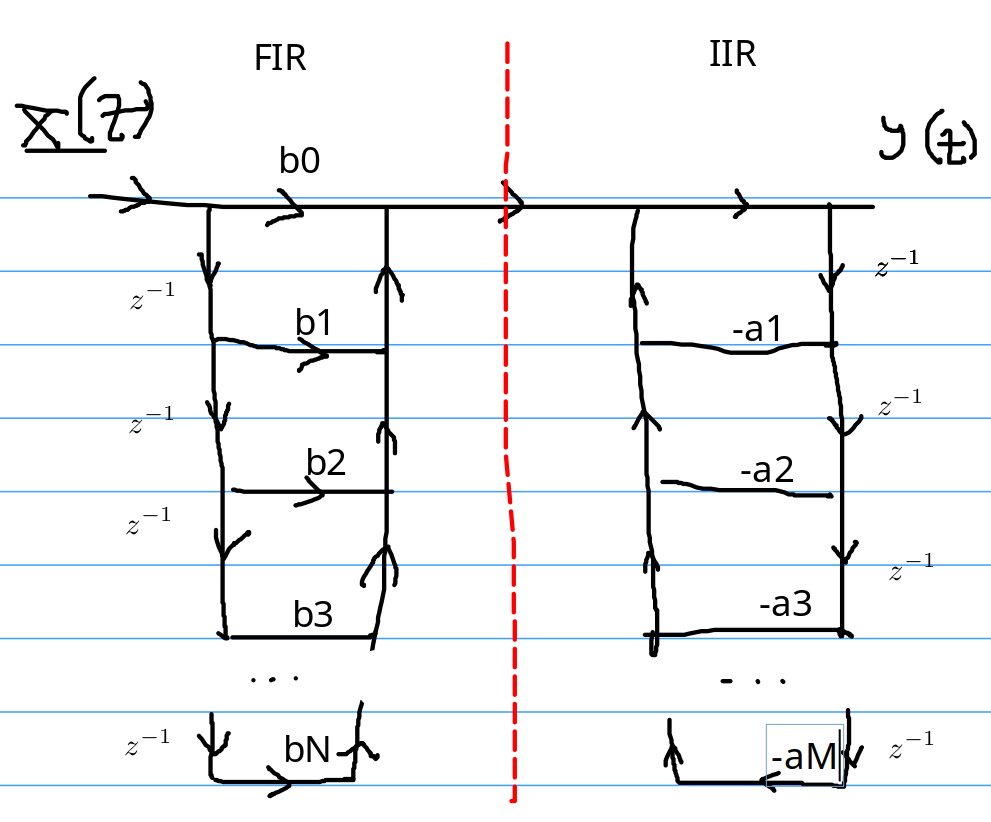
\includegraphics[width=16cm]{system.png}
  \end{center}
  \end{figure} 
\\Bộ lọc FIR là bộ lọc không hồi quy (không có phản hồi ngược lại), còn bộ lọc IIR là bộ lọc tự hồi quy (có phản hồi ngược lại từ đầu ra để feedback đầu vào).
Để tối ưu hóa tài nguyên, ta xây dựng kiến trúc hệ thống loại II, bằng cách \textbf{chuyển toàn bộ phần IIR sang bên trái và FIR sang bên phải} như sau:
\begin{figure}[H]
  \begin{center}
  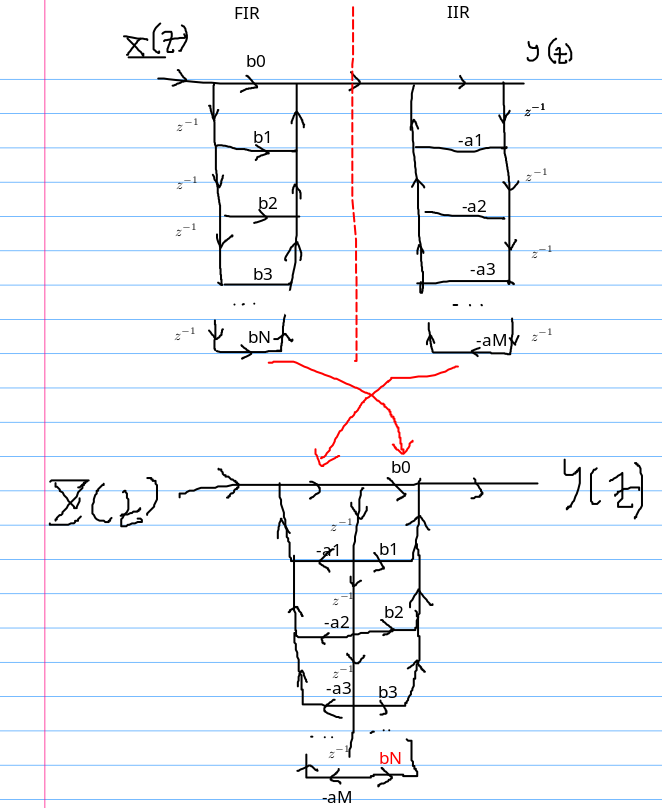
\includegraphics[width=10cm]{2..png}
  \end{center}
  \end{figure} 
\\ Vậy khi gặp cấu trúc hệ thống loại II, tốt nhất ta nên chuyển nó về loại I trước cho dễ nhìn, sau đó xây dựng phương trình sai phân biểu diễn hệ thống rồi làm gì thì làm. Cách chuyển đã được trình bày trên hình vẽ, chỉ cần "dịch" toàn bộ nửa bên trái sang bên phải và nửa bên phải sang bên trái là xong.
\section{Thiết kế bộ lọc FIR}

\subsection{Ý tưởng thiết kế bộ lọc FIR}
Ý tưởng của việc thiết kế bộ lọc FIR cực kì đơn giản như sau:
\begin{figure}[H]
  \begin{center}
  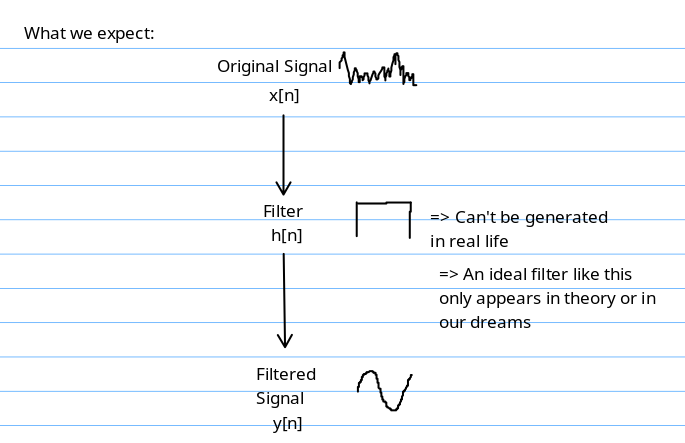
\includegraphics[width=16cm]{8.png}
  \end{center}
\end{figure}
\begin{figure}[H]
  \begin{center}
  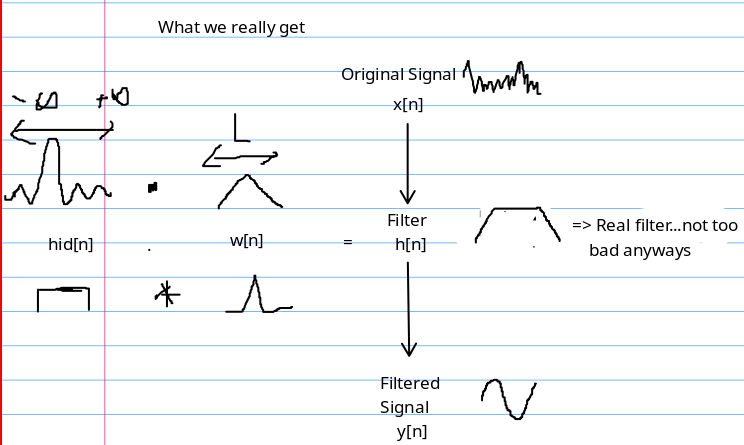
\includegraphics[width=16cm]{9.png}
  \end{center}
\end{figure}
\subsection{Thuật toán thiết kế bộ lọc LP:}
\begin{itemize}
  \item Tính tần số cắt $\omega_{c}$ hoặc $v_{c}$
  \item Tính đáp ứng xung lý tưởng $h_{id}[n]$
  \item Đọc thông số đề bài, chú ý đến $A_{s}$ và chọn cửa sổ, tính L
  \item Xây dựng hàm $h[n]=w[n]h_{id}[n]$
  \item Nhân quả hóa hàm $h[n]$
\end{itemize}
Ví dụ: Xác định đáp ứng xung của một bộ lọc LP lý tưởng có $\omega_{c}=\frac{\pi}{4}$ và thiết
kế bộ lọc FIR có hệ số $125$ bằng cửa sổ Blackman.
$$h_{id}[n]=\frac{1}{2\pi}\int_{-\pi}^{\pi}H(\omega)e^{j\omega n}d\omega=\frac{1}{2\pi}\int_{-\omega_{c}}^{\omega_{c}}e^{j\omega n}d\omega=\frac{\sin(\omega_{c}n)}{n\pi}$$
Thay $\omega_{c}=\frac{\pi}{4}$, xong:
$$h_{id}[n]=\frac{\sin({\frac{\pi}{4}n})}{n\pi}$$
Hệ số $125$, tức là $L=125$. Ta suy ra đáp ứng xung của bộ lọc dùng cửa sổ Blackman với hệ số $L=125$ là:
$$h[n]=h_{id}[n]w_[n] \quad |n|\leq\frac{L-1}{2}$$
Cuối cùng, ta chuyển bộ lọc về bộ lọc nhân quả bằng cách dịch bộ lọc đi.
$$h_{NQ}[n]=h\left[n-\frac{L-1}{2}\right]=h_{id}\left[n-\frac{L-1}{2}\right]w\left[n-\frac{L-1}{2}\right]$$
\subsection{Thuật toán thiết kế bộ lọc HP:}
Dựa trên phổ của bộ lọc LP và HP, ta có nhận xét sau:
\begin{equation}
  H_{HP}(\omega)=1-H_{LP}(\omega)
\end{equation}
\begin{equation}
  H_{HP}(\omega)=H_{LP}(\omega-\pi)
\end{equation}
Với hai cách biểu diễn phổ của bộ lọc HP như trên, ta có 2 thuật toán tương ứng để chuyển từ bộ lọc LP sang HP tương ứng.
\begin{enumerate}
  \item Thiết kế bộ lọc $h_{LP}[n]$ với tần số cắt $\omega_{c}=(\omega_{s}+\omega_{p})/2$, sau đó chuyển về bộ lọc HP qua phương trình:
  $h_{HP}[n]=\delta(n)-h_{LP}[n]$, sau đó dịch về nhân quả.
  \item Thiết kế bộ lọc $h_{LP}[n]$ với tần số cắt $\omega_{c}=\pi-[(\omega_{s}+\omega_{p})/2]$, sau đó chuyển về bộ lọc HP qua phương trình:
$h_{HP}[n]=(-1)^n h_{LP}[n]$, sau đó dịch về nhân quả.
\end{enumerate}
Trong thực tế thường người ta sẽ hay dùng cách (2) hơn vì tạo ra xung $\delta(n)$ khá khó.
\subsection{Thuật toán thiết kế bộ lọc BP:}
Dựa trên phổ của bộ lọc LP, ta sẽ dịch phổ của bộ lọc LP về hai phía là thu được bộ lọc BP dễ dàng.
\begin{figure}[H]
  \begin{center}
  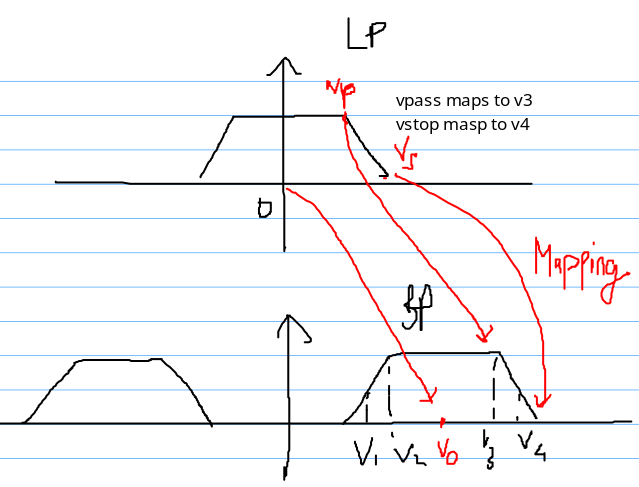
\includegraphics[width=16cm]{map.png}
  \end{center}
\end{figure}
Thuật toán thiết kế như sau: 
\begin{itemize}
\item Đổi tất cả các tần số về tần số số
\item Tính các tần số sau:
$$v_{0}=\frac{v_{2}+v_{3}}{2}=\frac{v_{1}+v_{4}}{2}$$
$$v_{s}=v_{3}-v_{0}$$
$$v_{p}=v_{4}-v_{0}$$
$$v_{c}=\frac{v_{s}+v_{p}}{2}=\frac{v_{3}+v_{4}}{2}-v_{0}$$
\item Thiết kế bộ lọc $h_{LP}[n]$ tương ứng với các thông số đã cho
\item Dịch bộ lọc $h_{LP}[n]$ bằng phương trình:
$$h_{BP}[n]=h_{LP}[n]2\cos{(2v_{0}n)}$$
\end{itemize}
\subsection{Thuật toán thiết kế bộ lọc BS}
Dựa trên phổ của bộ lọc BP, ta chỉ lấy phần bù, tức là:
$$H_{BS}(\omega)=1-H_{BP}(\omega)$$
là xong.
\end{document}
